\documentclass{article}[11pt]
\usepackage[top=1in,bottom=1in,left=1in,right=1in]{geometry}
\usepackage{setspace}
\usepackage{amsmath}
\usepackage{amsthm}
\usepackage{amssymb}
\usepackage{stmaryrd}
\usepackage{enumitem}
\usepackage{times}
\usepackage{graphicx}
\usepackage{latexsym}
\usepackage{bussproofs}
\usepackage{MnSymbol}
\usepackage{wasysym}
\usepackage{turnstile}
\usepackage{pgf}
\usepackage{adjustbox}% http://ctan.org/pkg/adjustbox
\usepackage{xcolor}
\usepackage{gensymb}
\usepackage{titlesec}
\usepackage{pdfpages}
\usepackage[hidelinks]{hyperref}
\usepackage[autostyle]{csquotes} 
\usepackage[doi=false,useprefix=true,isbn=false,url=false,style=chicago-authordate,natbib=true,]{biblatex} 
 
\defbibheading{bibliography}{}

 
\addbibresource{KMR_Master.bib} 

\DeclareMathSymbol{\Gamma}{\mathalpha}{operators}{0}
\DeclareMathSymbol{\Delta}{\mathalpha}{operators}{1}
\DeclareMathSymbol{\Theta}{\mathalpha}{operators}{2}
\DeclareMathSymbol{\Lambda}{\mathalpha}{operators}{3}
\DeclareMathSymbol{\Xi}{\mathalpha}{operators}{4}
\DeclareMathSymbol{\Pi}{\mathalpha}{operators}{5}
\DeclareMathSymbol{\Sigma}{\mathalpha}{operators}{6}
\DeclareMathSymbol{\Upsilon}{\mathalpha}{operators}{7}
\DeclareMathSymbol{\Phi}{\mathalpha}{operators}{8}
\DeclareMathSymbol{\Psi}{\mathalpha}{operators}{9}
\DeclareMathSymbol{\Omega}{\mathalpha}{operators}{10}


\DeclareFontFamily{U} {MnSymbolA}{}

\DeclareFontShape{U}{MnSymbolA}{m}{n}{
  <-6> MnSymbolA5
  <6-7> MnSymbolA6
  <7-8> MnSymbolA7
  <8-9> MnSymbolA8
  <9-10> MnSymbolA9
  <10-12> MnSymbolA10
  <12-> MnSymbolA12}{}
\DeclareFontShape{U}{MnSymbolA}{b}{n}{
  <-6> MnSymbolA-Bold5
  <6-7> MnSymbolA-Bold6
  <7-8> MnSymbolA-Bold7
  <8-9> MnSymbolA-Bold8
  <9-10> MnSymbolA-Bold9
  <10-12> MnSymbolA-Bold10
  <12-> MnSymbolA-Bold12}{}

\DeclareSymbolFont{MnSyA}{U}{MnSymbolA}{m}{n}
\DeclareMathSymbol{\twoheaduparrow}{\mathop}{MnSyA}{25}
\DeclareMathSymbol{\twoheadrightarrow}{\mathop}{MnSyA}{24}

\makeatletter

% % % % % % % % % % % % % % % % Footnote Command % % % % % % % % % % % % %
\usepackage{refcount}% http://ctan.org/pkg/refcount
\newcounter{fncntr}
\newcommand{\fnmark}[1]{\refstepcounter{fncntr}\label{#1}\footnotemark[\getrefnumber{#1}]}
\newcommand{\fntext}[2]{\footnotetext[\getrefnumber{#1}]{#2}}

% % % % % % % % % % % % % % % Internal Commands NMC% % % % % % % % % % % % %
\newcommand{\raisemath}[1]{\mathpalette{\raisem@th{#1}}}
\newcommand{\raisem@th}[3]{\raisebox{#1}{$#2#3$}}

\newcommand{\uuparrow}{% 
	\raisebox{.165ex}{\clipbox{0pt .6pt 0pt 0pt}{$\uparrow$}}
}
\newcommand{\tuuparrow}{% 
	\raisebox{.165ex}{\clipbox{0pt 1pt 0pt 0pt}{$\scriptscriptstyle\uparrow$}}
}
\newcommand{\muparrow}{% 
	\raisebox{.05ex}{\clipbox{0pt .65pt 0pt 0pt}{$\scriptstyle\uparrow$}}
}
\newcommand{\Uuparrow}{% 
	\raisebox{.2ex}{\clipbox{0pt .15pt 0pt 0pt}{$\Uparrow$}}
}
\newcommand{\thuarrow}{% 
	\raisebox{.05ex}{\clipbox{0pt .8pt 0pt 0pt}{$\twoheaduparrow$}}
}

% % % % % COMMANDS FOR NON-MONOTONIC CONSEQUENCES % % % % % % % % %
\newcommand{\nms}{%
	\mathbin{\mathpalette\@nms\expandafter}
}
\newcommand{\@nms}{\mid\joinrel\mkern-.5mu\sim}


\newcommand{\nmc}{%
	\mathbin{\mathpalette\nm@\expandafter}
}
\newcommand{\nm@}{\mid\joinrel\mkern-.5mu\sim\mkern-3mu}

\newcommand{\qmc}[1]{\mathrel{
		\mathchoice
		{\normalsize\hspace{.4mm}\nms^{\mkern-18mu\scriptsize\uuparrow#1}\hspace{-.7mm}}
		{\normalsize\hspace{.4mm}\nms^{\mkern-18mu\scriptsize\uuparrow#1}\hspace{-.7mm}}
		{\footnotesize\hspace{.4mm}\nms^{\mkern-13mu\tiny\uuparrow#1}}
		{\scriptsize\nms^{\mkern-10mu\tiny\tuuparrow#1}}
	}
}

\newcommand{\mqmc}{\mathrel{
		\mathchoice
		{\hspace{.4mm}\nms^{\mkern-18mu\scriptsize\uuparrow}\hspace{.6mm}}
		{\hspace{.4mm}\nms^{\mkern-18mu\scriptsize\uuparrow}\hspace{.6mm}}
		{\footnotesize\hspace{.4mm}\nms^{\mkern-11mu\tiny\uuparrow}\hspace{.6mm}}
		{\scriptsize\nms^{\mkern-10mu\tiny\tuuparrow}}
	}
}

\newcommand{\mrc}[1]{\mathbin{
		\mathchoice
		{\normalsize\hspace{.5mm}\nms^{\mkern-19mu\scriptsize\Uuparrow#1}\hspace{-.5mm}}
		{\normalsize\hspace{.5mm}\nms^{\mkern-19mu\scriptsize\Uuparrow#1}\hspace{-.5mm}}
		{\footnotesize\hspace{.5mm}\nms^{\mkern-13.5mu\fontsize{5.5}{0}\Uuparrow#1}}
		{\scriptsize\nms^{\mkern-10mu\tiny\Uuparrow#1}}
	}
}

\newcommand{\smc}{\mathbin{
		\mathchoice
		{\hspace{.4mm}\nms^{\mkern-17mu\scriptsize\thuarrow}\hspace{.6mm}}
		{\hspace{.4mm}\nms^{\mkern-17mu\scriptsize\thuarrow}\hspace{.6mm}}
		{\footnotesize\hspace{.4mm}\nms^{\mkern-11mu\tiny\thuarrow}\hspace{.6mm}}
		{\scriptsize\nms^{\mkern-10mu\tiny\thuarrow}}
	}
}
\newcommand{\nnmc}{\not\nmc}
\newcommand{\nsmc}{\not\mkern-3mu\smc}
\newcommand{\nmrc}{\not\mkern-3mu\mrc}
\newcommand{\nmqmc}{\not\mkern1mu\mqmc}
\newcommand{\nqmc}{\not\mkern1mu\qmc}

\newcommand{\nme}{%
	\mathbin{\mathpalette\@nme\expandafter}
}
\newcommand{\@nme}{{\mid\joinrel\mkern-.5mu\sim\mkern-2mu}_{e}\mkern3mu}


%\newcommand{\nme}{\nms\mkern-7mu_{e}\mkern2mu}
\newcommand{\qme}{{\qmc\mkern-2mu}_{e}\mkern3mu}
\newcommand{\mqme}{{\mqme\mkern-2mu}_{e}\mkern3mu}
\newcommand{\sme}{{\smc\mkern-2mu}_{e}\mkern3mu}

% % % % % % % % % % %Commands for Material Incoherence% % % % % % % % % % % %

\newcommand{\bigperpp}{%
	\mathop{\mathpalette\bigp@rpp\relax}%
	\displaylimits
}
\newcommand{\bigp@rpp}[2]{%
	\vcenter{
		\m@th\hbox{\scalebox{\ifx#1\displaystyle1.3\else1.3\fi}{$#1\perp$}}
	}%
}
\newcommand{\bigperp}{\raisemath{.5pt}{\bigperpp}}

%% % % % % % Degree Command % % % % % % % % % % % % % % % % % % % %
\renewcommand{\degree}{\ensuremath{^\circ}}


% % % % % % % % % % % % % % %%Macros for section title format % % % % % % % % % % % % %
%
\titlespacing{\section}{0pt}{*0}{*2}

\titleformat{\section}% These commands define the \section 
					[block]%  eliminates hanging indent for centered section
					{\large\bfseries\filcenter}% format commands
					{\thesection}%  Numbers sections
					{1ex}% separation between number and section title
					{}
					[]
					
\titlespacing{\subsection}{0pt}{*0}{*0}

\titleformat{\subsection}% These commands define the \subsection 
					[hang]%  default hanging indent 
					{\normalsize\bfseries}% format commands
					{\thesubsection}%  Numbers sections
					{1ex}% separation between number and section title
					{}
					[]
\titlespacing{\subsubsection}{0pt}{*0}{*0}
		
\titleformat{\subsubsection}% These commands define the \subsubsection 
					[hang]%  default hanging indent 
					{\normalsize\bfseries\itshape}% format commands
					{\thesection}%  Numbers sections
					{1ex}% separation between number and section title
					{}
					[]
					 
%this command sets the font to times new roman
\renewcommand*\rmdefault{ptm}

%commands for header
\usepackage{fancyhdr}
\pagestyle{fancy}
\rhead{Explanation and Scientific Inference}
\lhead{}

%opening
\title{}
\author{}
\date{}
\raggedbottom



\begin{document}
\doublespacing
\setlength{\parindent}{1cm}
\normalsize

\begin{center}
	\textbf{{\Large Explanation and Scientific Inference}}
\end{center}
\tableofcontents
\clearpage
%%%%%%%%%%%%%%%%%%%%%%%%%%%%%%%%%%%%%%%%%%%%%%%%%%%%%%%%%%%%%%%%%%%%%%%%%
%%%%%%%%%%%%%%%%%%%%%%%%%%%%%%%%%%%%%%%%%%%%%%%%%%%%%%%%%%%%%%%%%%%%%%%%%
\lhead{Significance and Impact}
\section{Significance and Impact}

%Inference to the best explanation (IBE) is a common pattern of inference in the sciences.  When a hypothesis is the best explanation of the available evidence, there is a strong reason to accept it.  We think that electrons exist because their existence explains a variety of electromagnetic and thermal phenomena.  Similarly, the best evidence for the theory of evolution is that it explains the fossil record.  Inference to the best explanation is ``inductive'' in the sense that the conclusion---that electrons exist, or that the theory of evolution is true---goes beyond the available evidence.  Induction presents longstanding philosophical puzzles. Contemporary discussion of inference to the best explanation concerns its status \textit{vis \capitalgrave{a} vis} other forms of inductive inference.  Can IBE be reduced to other forms of inference, or is it a fundamental form of inference in its own right? 
% 
%The status of IBE depends on an underlying account of explanation.  Arguably, none of the extant theories of explanation provides a strong basis for IBE.  Even worse, the views of explanation that link it closely to inference face daunting and unmet challenges.  Our project aims to develop a new account of explanation as a distinctive form of inference, and to use that account of explanation to understand the role of IBE in scientific inquiry.  The distinctive feature of our account of explanation is that it relies on developments in ``non-monotonic'' logic, where traditional accounts relied on classical logic as the underlying account of inference.  Non-monotonic logics more closely track the psychology of making inferences than classical logic, and they thereby more closely approximate scientific reasoning.  
%
%This project will have 

For Sherlock Holmes, the ``curious incident of the dog in the night-time''---its failure to bark---was a crucial piece of evidence.   He inferred that the mysterious midnight visitor was known to the dog.  Holmes' flights of reasoning typically took the form of explaining the clues he observed.  While Watson called the method ``deduction,'' it is known to contemporary philosophers as ``inference to the best explanation.''  Inference to the best explanation (IBE) is as common in science as it is in detective literature.  When a hypothesis is the best explanation of the available evidence, there is a strong reason to accept it.  For example, we think that black holes exist, at least in part, because their existence explains a variety of observed astronomical phenomena.

Inductive reasoning from observed evidence to laws and entities that cannot be observed is the distinguishing feature of scientific inquiry.  IBE is clearly a form of inductive inference, and the issue facing any purported form of inductive inference is reliability.  Under what conditions (if any) is it a reliable guide to the hidden structures of the universe? Different answers to this question have been proposed throughout the history of science, from outright skepticism about induction to enthusiasm about the power of statistics.  A variety of accounts of inductive inference have been proposed.  The relationship among these accounts is an outstanding issue in contemporary literature.  Induction is used across the sciences; does the reliability of inductive have different sources, or is a unified account of inductive inference possible?  One of the main attractions of IBE is that is applies to a wide variety of sciences, holding promise of a single account of inductive inference.

Understanding whether and why IBE is a reliable form of scientific inference requires both an account of explanation and an account of the relationship between inference and explanation.  Explanation has been a lively topic in the philosophy of science, but none of the extant theories of explanation provides a strong basis for IBE.  Those theories of explanation that best account for the reliability of IBE restrict it to a narrow range of sciences, while those theories of explanation that apply more broadly provide weaker bases for IBE.  Our project addresses this dilemma by developing a new account of explanation as a distinctive form of inference. 

Methodologically, this project differs from previous accounts of how inference is related to explanation. Where all previous accounts of explanation relied on classical logic and probability theory as the underlying account of inference, our project extends recent developments in non-classical logic. Our characterization more closely approximates scientific reasoning than does classical logic.  

Questions about explanation and inference strike deeply at our understanding of the scientific enterprise.  Skepticism about scientific rationality is often exacerbated by epistemologies that hold science to an idealized, external standard.  The logical innovations of this project highlight particular features of scientific practice and show why they are reliable.  By identifying explanation with particular kinds of scientific inference, we are able to account for the reliability of IBE in a way that captures the variety of explanations across the natural and social sciences.   

%Our project bases its account of the reliability of inference on scientific practice, using the strengths and weaknesses to circumscribe explanation and demonstrate the reliability of IBE. 



%The problematic in this domain has been to reconcile the rational character of science with its social dimensions.  Is science a reliable guide to the truth, or does it reflect social values and power dynamics?   The rationality of science suggests that it should be consensus-generating, while the pragmatic and political dimensions of scientific practice pull against consensus.  By grounding our account of the logic of explanation in the scientific practices of drawing inferences, we aim to show how this tension can be resolved.  Material inferences are shaped by the social context of scientific practice, including social values and pragmatics.  However, the robustness of an explanatory inference---the range of situations in which it holds---is not strictly a matter of choice or social convention.  The material with which we engage must cooperate too.  Our project thus illuminates the dynamic between social and material influences that constitutes science.


\clearpage

%%%%%%%%%%%%%%%%%%%%%%%%%%%%%%%%%%%%%%%%%%%%%%%%%%%%%%%%%%%%%%%%%%%%%%%%%
%%%%%%%%%%%%%%%%%%%%%%%%%%%%%%%%%%%%%%%%%%%%%%%%%%%%%%%%%%%%%%%%%%%%%%%%%

\lhead{Participants}
\section{List of Participants}

\noindent Khalifa, Kareem. Associate Professor of Philosophy, Middlebury College, Middlebury, Vermont.  \\[12pt]

\noindent Millson, Jared. Kirk Postdoctoral Fellow in Philosophy, Agnes Scott College, Atlanta, Georgia.  \\[12pt]

\noindent Risjord, Mark. Professor of Philosophy, Emory University, Atlanta, Georgia. \textbf{Project Director}  

\clearpage
%%%%%%%%%%%%%%%%%%%%%%%%%%%%%%%%%%%%%%%%%%%%%%%%%%%%%%%%%%%%%%%%%%%%%%%%%
%%%%%%%%%%%%%%%%%%%%%%%%%%%%%%%%%%%%%%%%%%%%%%%%%%%%%%%%%%%%%%%%%%%%%%%%%


\lhead{Narrative: Substance and Context}

\section{Project Narrative: Explanation and Scientific Inference}

\subsection{Substance and Context}
%(about ten pages)
%Provide a clear and concise explanation of the project and its value to scholars, students, and general audiences in the humanities. Describe the scope of the research, the source materials, the relationship of the research to other published and ongoing work in the field, and the major research questions to be addressed. Include a bibliographical essay that situates the project with regard to the existing relevant literature (and a bibliography of relevant primary and secondary sources in an appendix).

Scientific reasoning draws conclusions dramatically different from the evidence on which they are based.  Our knowledge of the function of DNA in the replication of phenotypic traits, for example, is not something that is directly observed.  Yet the theory is taken to be very well established.  The question of how such inductive inferences could be justified has been a central epistemic question about science since the scientific revolution.   David Hume (1711-1776) notoriously argued that induction was not a rational process; it was, rather, a habit of the mind.  Turning from the broad problem of justifying induction to the more tractable issue of distinguishing good inductions from bad ones, scientists and mathematicians like Thomas Bayes (1701--1761), Frances Galton (1822--1911), and Ronald Fischer (1890--1962) developed the understanding of probability and statistics that constitutes much of contemporary scientific inference.  It was another nineteenth century luminary, Charles Sanders Peirce (1839-1914) who suggested that the science required more than that the kind of generalizations captured by statistical inference.  While scholars debate the precise meaning of Peirce's ``abductive'' inference, contemporary philosophy  of science has developed Peirce's insight into the idea that explanatory power forms an important ground for scientific inference.

Studies of \textit{inference} to the best \textit{explanation} (IBE) stand at the nexus of the literatures on induction and scientific explanation.  The challenge, then, for any account of IBE is to satisfy both masters: to provide an account of inductive inference that shows why it is reliable, and an account of explanation that provides a satisfactory understanding of scientific inquiry.  Accounts of induction face a tension between reliability and breadth.  The most robust accounts of induction's reliability apply to the narrow range of sciences that admit of easy applications of statistical and probabilistic constructs.  The attraction of IBE as an account of inductive inference is its breadth, so if it is to be successful, it must provide a satisfactory account of induction's reliability. 

%ONe dilemma leads to another:  INduction trades off an account of reliability for breadth.  IBE uses explanation as its central concept.  Explanation trades off faithfulness to scientific practice for breadth.  Central dilemma: reliability vs breadth (driven by the concept of explanation) 

On the other hand, the main challenge facing theories of explanation is to provide an account that coheres with scientific practice.  Here the a trade-off is between breadth and accuracy.  The most accurate accounts of explanation fit best with a particular domain of scientific practice, and these are in the best position to provide IBE with an account of induction's reliability.  Those that apply widely admit too much and weaken the notion of explanation beyond recognition.  This pair of debates about induction and explanation converge to create a central dilemma for any account of IBE: an account of explanation that is sufficiently broad to underwrite IBE across the sciences requires a overly permissive account of explanation, while accounts of explanation robust enough to underwrite IBE are too restrictive to underwrite the full range of scientific inductions.  This project aims to design a new account of explanation that will be robust across the sciences, and thereby show how inference to the best explanation can be a reliable form of scientific inference.
%A central strand of debate about IBE has concerned its relationship to other forms of inductive inference.  The proponents of IBE hold that it is fundamental in the sense that it cannot be reduced to any other form of inductive inference. Critics of IBE argue either that explanation is too vague and permissive a notion to underwrite inductive inferences, or that IBE reduces to another form of inductive inference. 

%The attempt to characterize good inductive inference seeks to show that, \textit{contra} Hume, there are reliable ways to infer from observations to generalizations, causes, or entities too small or too large to observe.  In the twentieth century, optimism about the rationality of science has been dampened by a deepening understanding of the social dimensions of science.  Starting with Kuhn's \textit{Structure of Scientific Revolutions}, scholars across the humanities and social sciences have argued that science is shot through with politics and other social contingencies.  Contemporary scholarship on science has emphasized the integration of science with social interest by turning to study of scientific \textit{practices}, as opposed to theory. Explanation is not immune from this critique, since explanation is well know to depend on interest.  We select certain aspects of our environment for explanation, and the ways in which we explain them  often depend our interests in controlling the natural world and manipulating it for our purposes.  Inference to the best explanation is thus pulled between rational and social accounts of science.
%
%To meet the double challenge, our project begins with the scientific practice of drawing inferences.  The practices in view are the workaday inferences from ``The litmus paper turned red'' to ``The sample is acidic'' or from ``The patient tested positive for \textit{streptococcus} bacteria,'' to ``The patient has strep throat,'' as well as more elaborate, theoretical inferences.  The goal of both theories of induction and theories of explanation is to systematize these underlying inferences (what we will call \textit{material inferences}).  We do so by representing the inferences in a system of non-monotonic logic.  This allows us to isolate a class of particularly robust scientific inferences, which we identify with explanations.  Methodologically, our proposal about explanation is tested in two ways: by determining whether our representation of explanation is consistent with scientific practice (both contemporary and historical), and by comparing its strengths and weaknesses against other theories of explanation in the field.  
%
%With an account of explanation in hand, we can turn to the questions about inductive inference.  Unlike other theories of explanation, our account is naturally comparative; to determine that an inference is sufficiently robust to count as an explanation is already to compare it with the available competitors.  The method of testing our account of IBE is analogous to the test of the underlying account of explanation: by determining whether our representation of IBE licenses no inferences not already permitted in scientific practice, and by comparing our account of IBE to its competitors.



%The factors that motivate a pluralism of scientific approaches generates a wide variety of explanations to compare.  Choice of the most robust among the alternatives permits science to expand its explanatory power.

\subsubsection*{Contemporary Approaches to Inductive Inference}

A paradigmatic problem of inductive inference is to determine whether an observed sample is like the whole population.  If $46\%$ of polled voters say they will vote for a particular candidate, under what conditions can we conclude that the candidate will get $46\%$ of the actual vote?  Clearly, a conclusion about the whole population can never be certain, but are there ways to make the inference reliable? The challenge for an account of induction is to show that inductions can be reliable under some conditions, and explain the difference between reliable and unreliable inductions.  A further complexity in this field is that inductive inference appears in such a wide variety of forms and contexts: surveys, clinical trials, field observations, and so on.  This raises the question of whether there is a single account of induction that will assimilate all of these apparently different inferences, or whether inductive reasoning comes in many different, irreducible forms.


Contemporary answers to these questions divide accounts of inductive inference into two broad families:  Bayeseanism and hypothetical reasoning.  The first draws on the mathematics of probability theory to characterize the strength and reliability of inductive inferences.  The second family rose to prominence as the ``method of hypothesis'' during the 19th century.  It is grounded in a suspicion that the hidden structures of the world could not be simply read off of observed patterns or probabilities.  Rather, hypotheses must be invented and brought to the evidence for testing.

According to Bayesians, inductive reasoning consists of updating one's beliefs in accordance with Bayes' Theorem.  A central result of probability theory, Bayes Theorem shows how the probability of a hypothesis changes as new observations are made.  Bayeseans interpret this as showing how one's strength of belief in the truth of a hypothesis should increase or decrease in the light of new observation.  Each opinion poll, for example, is new evidence.  If one strengthens or weakens one's belief according to Bayes' Theorem (and the axioms of probability theory), one's degree of confidence in the hypothesis that a candidate will get $46\%$ of the vote will come to match the objective probability of the hypothesis.

Because Bayesianism is based on the mathematics of probability theory, it promises universal applicability.  Bayesianism works especially well when a rational agent's degrees of belief readily correspond to well-defined objective frequencies, such as coin tosses, opinion surveys, or radioactive decay. However, when these features are lacking, strict Bayesian approaches offer little guidance. For instance, the existence of intermediate species in the fossil records supports the theory of natural selection.  The relative frequency of such fossils seems to have little relevance to their evidential value.  Strict Baysean approaches thus has limited applicability: it trades off breadth for a clear and rigorous account of the reliability of inductive inference.


In response to this and other challenges, many Bayesians augment the probability calculus with further---and frequently controversial---assumptions.  In particular, by wedding the probabilistic machinery to graph theory, Bayesians have recently made substantial progress in the domain of causal inference (Pearl 2000; Spirtes, Glymour, and Scheines 2000). While powerful, these developments remain limited to a part of science. Not all scientific inquiry seeks causes, and many causal inferences are not easily represented with this Bayesian formalism.  So again, while these views give a clear account of why induction is reliable, they have limited application across the sciences.

The alternative, hypothetical family of approaches to inductive inference holds that scientific theories are not drawn out of the evidence, but are brought to it. Sir Karl Popper (1902-1994) proposed the most strident version of the hypothetical approach.  On his view, scientific reasoning consists of making (bold!) conjectures and testing them.  Popper followed Hume in rejecting the rationality of induction, and opposed the use of statistical inference to draw positive conclusions.  On his view, testing consisted only in the attempt to falsify a hypothesis, and the best we could say of our hypotheses is that they haven't been demonstrated false \textit{yet}.  While this view exhibits an admirable epistemic humility, it flies in the face of scientific practice, which takes evidence to provide positive support for theory.

Methodological textbooks often present a positive view of the conjecture-and-test account of induction.  On this view, a hypothesis and the threshold of statistical significance must be proposed \textit{prior} to making the observations. The hypothesis is accepted if it meets the threshold, and rejected otherwise.  In spite of its popularity in science pedagogy, conjecture-and-test is widely acknowledged to be an inadequate account of inductive inference all by itself.  Hypothesis acceptance is not an all-or-nothing matter.  Some account is needed to show how theories can be more or less well supported. Bayesians take this as reason to assimilate the conjecture-and-test method to their view. But like Bayesianism, conjecture-and-test applies poorly to some fields.  


Inference to the best explanation is a version of the hypothetical approach to inductive reasoning.  Like conjecture-and-test, it brings a hypothesis to the data.  But where conjecture-and-test uses the data to judge the acceptability or probability of the hypothesis, IBE tries to explain the data with a hypothesis.  IBE thus arguably strengthens the theory-evidence relationship by adding consideration of relative explanatory power.  While inferential statistics provides important tools, proponents of IBE argue that probability alone is a poor guide.  Hypotheses should be accepted not when they only meet statistical or probabilistic strictures, but when they are the best explanations of the data. In addition to providing a stronger account of inductive reasoning, proponents contend, IBE has the further advantage that it applies to a wider range of sciences than either its conjectural cousin or Bayesianism.  Since explanations are found across the sciences---including those that use qualitative methodologies---IBE seems to account for inductive reasoning in the broadest range of scientific practices.

Whether IBE can make good on its promise as an account of inductive inference depends on how ``best explanation'' is to be understood.  This requires an account of explanation and some kind of criteria for determining that one explanation is better than another.  Notoriously, most proponents of IBE provide only a thin notion of explanation and a relatively vague account of the theoretical virtues exhibited by the best explanation.  It is fair to say that these vagaries are both a blessing and a curse. On the one hand, because IBE is loosely defined, it is highly flexible, which is  where it outperforms other approaches. On the other hand, the leading criticisms of IBE stem precisely from this vagueness: the reliability of the virtues in arriving at the truth, the reducibility of IBE to other forms of inference, and the track record of IBE in the history of science.

When articulating criteria that make an explanation ``the best,'' proponents of IBE usually list a set of virtues, such as simplicity or conservatism. However, closer inspection of case studies from the history of science suggest that each virtue admits of multiple interpretations and that each virtue's weight relative to the other virtues varies according to context. (REF Khalifa, and add to bib) Moreover, many theoretical virtues appear to be merely of pragmatic or aesthetic value. Arguably, neither an explanation’s utility nor its elegance have much to do with its truth. Some have concluded that the pragmatic/aesthetic character of the virtues suggests that IBE is not a reliable form of inference.

A second objection to IBE also hinges on the aforementioned imprecision: its reducibility to more familiar forms of statistical inference.  Bayseans are the fiercest competitor here.  The best explanation, one might argue, needs to be the most probable of the alternatives.  Bayseanism provides a precise way to measure the probability of a hypothesis, given the current evidence.  Any inferential power of explanation, then is already contained in the Baysean probability calculations.  Some defenders of IBE have have fended off these reductions by arguing that there the different families of statistical and hypothetical inference are equiprimordial and complementary. However, absent a clearer sense of what the best explanation involves, even this irenic position---much less any reductive position---is difficult to evaluate.

The third challenge to IBE comes from the scientific realism debates. The history of science is replete with cases in which no true explanations were considered at a given time. Furthermore, our current situation could be no different than our predecessors’: we, too, could be failing to consider a true explanation and simply accepting the best of a bad lot. A frequent reply to these objections then strengthens the best explanation's requirements---demanding it to have predictive power or to cite mechanisms. However, this runs the risk of looking ad hoc, as many of our best explanations do not have these features.

A further challenge to IBE arises from a presupposition shared by all of the approaches to induction surveyed so far: the best way to understand induction is to determine its \textit{form}. John Norton (2003, 2007) has pointed out that this appeal to form misses crucial aspects of scientific inference.  For example, consider the following two inductive arguments:

\begin{quote} 
All observed examples of bismuth have melted at $271.5\degree$ Celsius. \\[-6pt] Therefore all bismuth melts at $271.5\degree$ Celsius.
\end{quote}

\begin{quote}
All observed samples of wax have melted at $91\degree$ Celsius. \\[-6pt]
Therefore all wax melts at $91\degree$ Celsius.
\end{quote}

\noindent Both arguments have the same form, usually called ``enumerative induction.''  However, only the first is a good inductive argument.  The reasons have to do with the subject matter.  Bismuth is an element, and that gives us substantial reason to believe that all samples will be similar with respect to their melting point.  Wax can be many different mixtures, and we expect them to have different melting points.  The material or content of the inference, not the form, determines the difference between good and bad inferences.

Norton is among a variety of scholars in the philosophy of science, philosophy of language, linguistics, and logic who have reversed the traditional priority of form over content.  In studies of induction, the consequence of this inversion is that the reliability of inductive arguments are not determined by their formal features. There may be important differences in the forms that inductive arguments take, but if we are to understand the conditions under which they will be reliable, we must attend to the background knowledge available about the subject matter of the inference.  Norton's account forfeits breadth insofar as the reliability of an inductive inference has to be evaluated locally, by attending to the details of what is known about the subject matter of the inference.  


Explanations depend on scientific background knowledge insofar as they draw on the theoretical context to explain a specific phenomenon.  IBE thus seems to be in a good position to exploit Norton's insight about induction.  However, theories of explanation have traditionally looked for a single form (or a small number of forms) that work across the sciences. Developing IBE so as to take advantage of Norton's insight requires a parallel account of explanation.  Our project aims to develop an account of explanation that will show how it depends on the local scientific context.  Since these contexts differ across the sciences, our account of explanation will achieve its breadth through the function of explanation in scientific practice,  not a unity of form.  Basing an account of explanation on scientific knowledge of the subject matter of explanation will be more precise than existing accounts of IBE.  It thereby holds promise for resolving the challenges to IBE that arise out of its vagueness. 


\subsubsection*{Theories of Explanation}

Any account of inference to the best explanation requires an understanding of \textit{explanation}. What are the defining features of an explanation? What distinguishes it from related phenomena, such as description, correlation, prediction, or classification? What makes one explanation better than another? As the previous section argued, without an antecedent grasp of what kinds of claims count as explanations in a given domain, and of how to evaluate those explanations, appeals to IBE are vague.  Many proponents of IBE have satisfied themselves with thin conceptions of explanation in order to achieve the necessary breadth for IBE's application.  Those who have adopted more substantive accounts of explanation have limited IBE's scope.  This is the central dilemma for any account of IBE: to provide an account robust enough to ground IBE's reliability, yet broad enough to apply across the sciences.  In spite of a vast literature, no existing analysis of explanation balances rigor with breadth in a way that adequately supports IBE.  

Accounts of explanation are commonly classified into three types: epistemic, causal, and pragmatic.  On epistemic accounts, something is explained when it is shown to fit a theory. A canonical epistemic account, Carl Hempel's ``covering law model,'' holds that explanations of an event or regularity show how it can be inferred from laws of nature and initial conditions.  For example, suppose a cue ball strikes a billiards ball, which then travels across the felt. To explain the latter's velocity, according to Hempel, we deduce the it's velocity from Newton's laws of motion and the initial velocity of the cue ball.  The successor to Hempel's account of explanation is the ``unification'' account of explanation.  Relaxing the requirement that all explanations appeal to laws, this view treats explanation as patterns of deductive inference that systematize scientific domains.

Historically, hypothetical accounts of induction have been paired with epistemic accounts of explanation. So, epistemic accounts are \textit{prima facie} promising as a foundation for IBE.  Hopes here are quickly dashed, for the adequacy of epistemic approaches has been challenged in many ways. First, they fail to preserve the asymmetry of explanation. In general, if $A$ explains $B$, then $B$ does not explain $A$.  From the cue ball's direction and velocity, we can calculate (and thereby explain) the billiards ball's direction and velocity.  But while we can do the reverse calculation, we do not thereby explain the motion of the cue ball.  The inferences are symmetrical, but the explanation is not.  Second, epistemic approaches fail to do justice to explanations of improbable events. For instance, biomedical researchers explain paresis by appeal to untreated syphilis, but only a quarter of untreated syphilitics develop paresis.  While having syphilis seems to explain why someone has paresis, the explanation does not fit the phenomenon to be explained within a wider regularity; improbable events are irregular.  For these and other reasons, epistemic approaches have fallen out of favor among philosophers of science, and no proponent of IBE has adopted this view.

Causal accounts take explanation to denote real relationships among things, rather than characteristics of a theory (such as the deductibility from laws, as in Hempel's account). On a causal account of explanation, to explain an event is to describe some part of its causal history.  The velocity of the cue ball thus explains the velocity of a billiards ball.  Treating explanation as a causal relationship rather than an inferential relationship immediately resolves the challenges facing epistemic accounts.  The velocity of the cue ball causes the velocity of the billiards ball, but not \textit{vice versa}; syphilis causes paresis, despite the low probability involved. Mechanistic accounts of explanation go further by demanding that explanations not only describe causal history, but show the mechanisms by which a phenomeon is brought about.  All varieties of causal account provide a detailed analysis of explanation, as well as clear criteria for what does and does not count as an explanation.  They do so, however, at the cost of breadth.  Causal accounts either have to deny that forms of scientific inquiry that do not seek causes or mechanisms are non-explanatory, or leave the analysis of such explanations to other theories.


Some of the most prominent articulations of IBE, such as Peter Lipton's (2004), use a causal account of explanation as the basis for a view of IBE.  While Lipton gives a good account of why IBE is a reliable form of inductive inference, it is subject to two problems.  First, there are scientific explanations that do not invoke causes.  By basing IBE on an analysis of explanation limited to causality, proponents of IBE must abandon broader claims about IBE in scientific reasoning.  Moreover, the discovery of causes is itself a form of inductive reasoning. Many causal explanations depend on a prior grasp of non-explanatory, inductive inference.  By accepting a causal account of explanation, proponents of IBE potentially cede large swaths of the battlefield to the Bayesians.    

The third kind of theory of explanation is pragmatic.  These accounts take explanations to be answers to questions asking ``Why\dots ?''. Since why-questions arise in all scientific fields, as well as in the humanities, the pragmatic accounts  have the broadest scope of the three alternative views of explanation.  Questions are a form of speech act, that is, actions performed through the use of words.  As such, questions are highly context sensitive. The practical or scientific interests of the person asking the question deeply affect the range of acceptable answers. One phenomenon can be the subject of many why-questions, and while the answers are different, they need not conflict. The diversity of scientific interests thus motivates a pluralistic attitude toward scientific inquiry.  And since questions are inter-personal, pragmatic accounts fit naturally into a picture of science as a social enterprise.  Despite this greater coverage, pragmatic approaches face many of the same problems bedeviling epistemic accounts.  For example, they fail to capture explanatory asymmetries, since we can use the billiards ball's velocity to answer the question why the cue ball had a given velocity. Additionally, pragmatic approaches weaken the connection between explanation and inference. Indeed, the pragmatic approach's most prominent proponent, Bas van Fraassen (1980) used it to argue \textit{against} IBE. The otherwise attractive breadth leaves us with too many explanations and no way to choose the ``best'' in a manner that promotes good scientific inference.

Inference to the best explanation, then, is a pervasive form of reasoning that \textit{appears} to have a central role in science.  Considered as a distinct, even fundamental, form of inductive inference, IBE has significant advantages over the alternative accounts of inductive reasoning.  However, IBE has been damaged by the lack of a suitable account of its central concept: explanation.  Remaining agnostic about this central idea leaves the view open to objections and to the reduction of IBE to other forms of inference.  Choosing one of the alternative accounts of explanation returns us to the central dilemma facing any account of IBE.  Causal accounts of explanation are currently popular among philosophers of science because they capture in an articulate way some central aspects of scientific practice.  By doing so, they abandon the attempt to be comprehensive.  The pragmatic accounts are sufficiently broad to apply to all kinds of scientific inquiry, but they are too permissive about what is to count as an explanation, and they fail to show why IBE is a reliable form of inductive inference.  This project proposes to develop an account of explanation that applies to the full range of explanatory practices in science, but does so in a way that discriminates between explanatory inferences (e.g. the cue ball's velocity explains the billiards ball's velocity) and non-explanatory inferences (e.g. the billiards ball's velocity explains the cue ball's velocity).  In the light of such a conception of explanation, we will be in a position to understand  whether (and under what conditions) IBE is a reliable form of scientific inference.


\subsubsection*{Explanation as Inferential Practice}


%As we have seen, none of the three approaches to explanation can provide IBE with what it needs. Pragmatic approaches are too permissive to faithfully track scientific explanations; causal approaches are too restrictive; and neither provides a notion of explanation that would render IBE a cogent and interesting form of inference. Epistemic approaches might well solve this last problem, but they end up being too permissive in some places and too restrictive in others. To navigate this minefield of difficulties, we offer a new position that is both epistemic and pragmatic: an \textit{inferential practice} account of explanation.
Norton's critique of induction was that the reliability of inductions did not depend on their deployment of a particular form.  Rather, the content of the inference determined whether it was good.  We suggest that a similar problem lies at the root of the difficulties surrounding explanation and IBE.  Epistemic theories of explanation are promising as the basis for IBE because they propose a close relationship between inference and explanation.  However, all epistemic theories of explanation so far have followed the tradition of classical logic and prioritized form over content.  Something is an explanation, on the epistemic views, only if it fits a particular logical form, such as a mathematical calculation from laws. Our project will develop a new epistemic account of explanation that inverts the traditional priority of form over content.  By doing so, our epistemic theory can resolve the longstanding issues that have put epistemic theories of explanation into disfavor.


%Following Norton's lead, we suggest that the root of the difficulties that surround explanation and inference, we suggest, is they have thought about inference in the wrong way.  Both traditional accounts of induction and the epistemic approaches to explanation have assumed that inference is a \textit{formal} relationship between sentences in a language.  This means that we can represent all good inferences as sharing a form or template, into which different material can be inserted.  Enumerative induction, for example, is often represented as the form ``All observed samples of $F$ have been $G$, therefore All $F$s are $G$.''  In this template, $F$ and $G$ are properties, such as being bismuth and having a melting temperature of $271.5\degree$ Celsius.  If it is true that every observed sample of bismuth has had a melting temperature of $271.5\degree$ Celsius, then the template of enumerative induction licenses the inference that bismuth melts at $271.5\degree$ Celsius.  


Because all previous epistemic theories of explanation  have used classical, deductive logic and probability theory as their underlying account of inference, they have prioritized form over content.  By contrast, our epistemic theory of explanation will prioritize content over form.   In logic, prioritizing content over form means that the goodness of an inference does not depend on the arrangement of logical operators like ``if \dots then'' or ``all.''  Such logical operators and  rules are important because they serve to highlight or express the underlying relationships, and they allow us to endorse or criticize kinds of inference.  The force of the reasoning is carried by the underlying inferential relationships called ``material inferences.''  For example, in many contexts, the following inference would be judged as good without any additions:

\begin{quote}
The litmus paper turned red. \\[-6pt]
Therefore, the liquid was acidic.	
\end{quote}

\noindent Classical logic, by contrast, would not regard this inference as valid without the addition of a premise like ``If the litmus paper turns red, then the liquid is acidic.''  An important trend in contemporary logic is to show how the properties of formal operators like ``if. \dots then'' can be constructed from material inferences like the one above (Brandom 2004, Peregrin REF). 

In the philosophy of science, the priority of content over form means prioritizing scientific practice.  Whether an inference is good or bad is based on information about the subject matter---about acid and litmus paper---not a matter of fitting it into a logical framework like enumerative induction or Bayes Theorem.  Material inferences in a scientific context are those judged to be good or acceptable in the light of the established science of a given domain.  Our approach to explanation and IBE takes material inferences as its starting point.

Treating material inference as prior to formal inference has two significant consequences for understanding science.  In \textit{Natural Laws in Scientific Practice} (2000) and subsequent writing, Marc Lange has developed the first.  Lange has shown the importance of the implicit ``modal'' character of material inference.  To infer that the liquid is acid because the litmus paper turned red is to implicitly accept a range of possibilities: that the paper would not have turned red on its own, that it would have been blue if the liquid was a base, and so on.  The modalities of necessity and possibility are already built into the scientific understanding that supports the inference.  Lange shows how the necessity of both natural and mathematical laws can be built from the implicit modality of material inferences. 

The second consequence is that material inferences are sensitive to changes in the available  information in ways that most logical forms used by traditional epistemic theories of explanation are not.  Traditional philosophy of science took deductive logic to provide the paradigm for scientific inference.  Classical, deductive logic is ``monotonic'' in the  sense that additions to the premises do not undermine the validity of the inference.  For example, the following is a classically valid argument:

\begin{quote}
	If the litmus paper turned red, then the solution is acidic. \\[-6pt]
	The litmus paper turned red. \\[-6pt]
	Therefore the solution is acidic
\end{quote}

\noindent Suppose we learned that the litmus paper had been dipped into a can of red paint.  According to classical logic, the argument would remain valid even if we added this new information.  In real scientific reasoning, however, the addition of this information would disrupt the inference: we would no longer draw the conclusion that the solution was acidic.  This means that the forms of classical logic are a poor representation of scientific reasoning.  For our project, the material inferences of scientific practice are \textit{non-monotonic}.

A central part of the methodology of our research is to find ways to precisely identify and represent the material inferences of scientific practice.  Our approach draws on both Lange's insight and recent work on non-monotonic logic.   There is a range of possibilities within which the inference ``the litmus paper turned red, therefore the solution is acidic''  remains scientifically acceptable.  That range includes the possibility that the scientist was Swedish, or that the test took place on a Tuesday.  Importantly, it excludes the possibility that the test was conducted on a can of red paint, or that the litmus paper was defective.  Every material inference is surrounded by a kind of ``island of stability,'' composed of possibilities consistent with the inference. Indeed, an important part of scientific research is to establish the limits of such islands of stability around important hypotheses.  In our research so far, we have given a precise characterization of what is here figuratively called the ``island of stability.''   A consequence of this characterization is that we developed criteria for comparing such islands, and thus comparing the relative stability of material inferences. 

We propose that explanations are those material inferences that remain acceptable under the widest range of possibilities.  When an inference like ``the litmus paper turned red  because the liquid was an acid'' is called an ``explanation,'' we are expressing a commitment to the stability of the inference.  It is more stable---has a larger ``island''---than any alternative inference with the same conclusion. In a forthcoming paper, we show that this permits us to solve the symmetry problem, which plagued earlier epistemic and pragmatic accounts of explanation.  The red of the litmus paper does not explain why the liquid is acidic, but the acid does explain why the paper turned red.  On our account, the first inference is not an explanation because there are other ways to infer the liquid's acidity (e.g. a story about how it was distilled) that are compatible with a wider range of possibilities.  

For an inference to be maximally stable,  it must be compatible with a wider range of possibilities than any competitor.  This means that the most stable inference---the explanation---will include all of the factors relevant to a phenomenon. The conception of explanation just sketched, then, identifies criteria for a complete or total explanation. Practically speaking, however, we are often interested in only one part of the complete story. Following pragmatic theorists of explanation, we argue that what makes one explanation the ``best'' is partly a contextual matter.  For neuroscientists, for example, the best explanation of a person’s pain will invoke neurons and ion channels; for doctors, a description of a recent injury will often be better. On our view, pragmatic considerations license selecting one part of a complete explanation and treating it as the best in a given context.  Inference to the best explanation, then, has an ineliminable pragmatic dimension. Because this pragmatics is built on the foundation of a robust semantics for ``explains,'' our account is not as permissive as the standard pragmatic accounts of explanation.

Our new account of explanation provides a new foundation for IBE.  An adequate account of IBE must provide criteria for the choice of the \textit{best} explanation, and show why it is that explanatory inferences are reliable.  As developed so far, our account of explanation shows promise on both counts.  An explanation, we propose, is an inference with more stability than any other inference to the same conclusion.  This criteria identifies one set of factors as explanatory.  Within a single set of explanatory factors (the total explanation), pragmatic considerations determine the selection of one aspect as the most relevant to our interests at the time.  Our account of explanation thus naturally yields a best explanation in a given context.  When we have an explanation in hand, it will be modally robust in the sense that it remains acceptable under a range of possible circumstances.  Indeed, the best explanation will have the \textit{widest} range of stability.  The reliability of an inference to the best explanation will depend on the circumstances.  As long as we have reason to believe that we are not in conditions that would undermine the inference (that is, we are not ``off the island''), the inference remains scientifically acceptable.  Applied to specific inferences, we can specify the conditions under which IBE is and is not a reliable form of inference.


To resolve the central dilemma facing any account of IBE, we must show that our account of IBE is robust across the full range of the sciences.  This means that our conception of explanation must fit a wide variety of examples of explanatory practice.  To guarantee that our view does so, we will use a case study methodology. We will select events from the history of science or contemporary science where scientists developed new explanations.  We will read the journal publications and other research notices to determine the variety of possible inferences and explanations explored by the scientists.   We will then modify our view as necessary to capture the character of their reasoning.  


We will conduct cases studies in the following areas: asymptotic explanations in thermodynamics, Gell-Mann and Ne'eman's classification of baryons and mesons (the so-called ``Eightfold Way''), the modern synthesis of natural selection and genetics, contemporary theories of pain, the discovery of bacterial causes for ulcers, and structural explanations in the social sciences.  These cases satisfy several desiderata. They are drawn from a full representation of the natural and social sciences, and they capture some of the variation within fields.  In addition, they represent a mix of cases previously discussed in the philosophy of science and new examples. Those that have been previously discussed provide points of comparison with competitors to our accounts of explanation and IBE.  The new cases let us test our view against a wide range of scientific practices.  

In addition to the case studies, we will support our account by showing that it provides satisfactory answers to the outstanding questions in the literature on IBE and explanation.  With respect to the explanation literature, there are a number of well known problem cases for any theory of explanation.  The symmetry problem and the problem of explaining improbable events, mentioned above, are two well known puzzles.  The first test of our nascent account, then, will be to see whether it handles the troublesome cases in the explanation literature.  That our view can account for the asymmetries of inference, while no other epistemic account of explanation could do so, is an important preliminary result.   As we tackle the other problematic cases, we may need to further revise our initial account of explanation as maximally stable inference.

With respect to the literature on IBE, our conception of explanation permits us to address two central questions: whether IBE is fundamental, and whether it is a guide to the truth.  Our answers to both challenge the terms in which these questions have been discussed. The question of IBE's fundamentality has been conducted in terms of \textit{reduction}: Can IBE be reduced to Bayesianism or some other philosophical account of induction?  This debate prioritized form over content, and inquires into the relationship among formal representations of inference.  On our view, material inferences are primary, and explanations express particularly important kinds of inference.  While there is an important sense in which IBE is not fundamental (material inferences are primary), neither can IBE be assimilated to competing theories of inductive inference.  

Whether a particular inference to the best explanation is a guide to truth, on our view, depends on the underlying material inferences.  Their reliability is not something that can be determined \textit{a priori} by philosophical theory.  Sorting good from bad material inferences is a matter of ongoing scientific inquiry.  Our account highlights the points where scientific criticism is most relevant to evaluating inferences to the best explanation.  In particular, the range of circumstances under which an inference remains stable is an important scientific question, and on our account, such stability is directly relevant to the reliability of an IBE.   From this point of view, then, IBE is reliable in those scientific domains that are well established, but not always in those domains that remain scientifically uncertain.  


\lhead{Narrative: History of the Project}
\subsection{History of the Project and its Productivity}

%about three pages)
%Provide a history of the project to date. Explain how the 
%project began, its progress, and its estimated date of completion. Describe any research or planning that has already been completed , and the resources or research facilities available. In table format list any print or digital products with dates of publication; when applicable, the list must indicate the publisher, print or production runs, and usage statistics. 

\lhead{Narrative: Collaborators}
\subsection*{Collaborators}

%three pages
%Name the project director and all collaborators who would work on the project during the proposed grant period, regardless of whether NEH funds are requested to support their participation in the project. Describe their responsibilities and qualifications. State anticipated commitments of time for the project director and all collaborators, and explain the reasons for and nature of their participation.Project directors must devote a significant portion of their time to their projects. Provide résumés of the principal collaborators (maximum of two pages each) in an appendix.

Dr. Kareem Khalifa is an associate professor of Philosophy at Middlebury College. He has written several articles on the topic of explanation, and has a forthcoming book, \textit{Understanding, Explanation, and Scientific Knowledge} (Cambridge University Press), in which he argues that our understanding of empirical phenomena is a function of our explanatory knowledge. Dr. Khalifa brings to the project an expertise in epistemology and general philosophy of science. He has defended pragmatic views of explanation, and a deflationary view of IBE's import to realism.

Dr. Jared Millson is a Kirk Postdoctoral Fellow in Philosophy at Agnes Scott College. In his dissertation, \textit{How to Ask a Question in the Space of Reasons}, he argued that the ability to ask and answer questions is a necessary component of any linguistic practice. In defending this claim, he developed a novel dynamic pragmatics for questions that will be the basis for our work in Chapters 2 and 3. He has used this theory to construct a formal-logical model of question-answer exchanges. He brings to the project substantial expertise in logic, linguistics and philosophy of language.

The Project Coordinator, Dr. Mark Risjord is a professor of Philosophy at Emory University. In his first book, \textit{Woodcutters and Witchcraft} he developed a pragmatic theory of explanation and an account of inference to the best explanation. Risjord has also written about the role of political values in choice of explanation, and specifically on the issue of the explanatory power of the race in anthropology and medicine. The current project substantially revises and extends this earlier work. 

\lhead{Narrative: Methods}
\subsection{Methods}

%four pages
%Explain howthe p roject’ interpretive goals correspond to the proposed methodology. 
%
%Explain how central research questions will be approached and how any 
%potential difficulties in working with primary source materials will be 
%resolved.
%
%Describe in detail the tasks to be undertaken and the digital technology to be employed, indicating what resources will be required, as well as the experience of the collaborators with the technology and its application to humanities scholarship. If your project involves a large amount of data, describe your plan to manage the data
\subsubsection*{Writing Process}

All of our writing is the result of forming a consensus through criticism and revision.  The drive to find consensus in the face of opposing arguments forces each of us to modify our views.  As a result, we feel the final product is philosophically stronger than what any of us could achieve alone.  Authorship attribution is therefore equal, and authors are listed alphabetically in publications.  Where one of the authors is primarily responsible for a particular result (especially formal results in our logical investigations), it is noted in the acknowledgments. 

Our collaborative process proceeds through four methodological phases.  First, we conduct a literature review of a chapter’s relevant topic, guided by the member of the team with the most background. After working through the literature, we debate where we stand within the relevant dialectic until consensus is reached on the broad outline of the position we want to adopt. From there, we identify our burdens of proof. For instance, because our view treats explanations as inferences, we need to show how it preserves earlier inferential approaches' strengths, while avoiding their weaknesses. This is frequently clarified by reconstructing  and critiquing the arguments in the literature, and then modifying our position in response to the strongest arguments. 

Second, the methodological novelty of the work has been to extend recent literature in semantics and pragmatics to the special case of explanations and why-questions in science. Millson has been primarily responsible for marshaling resources from contemporary linguistic and logical theory to build a formal model of explanatory inferences. Chapter 2's model is largely complete. Chapter 3's model builds on independent earlier work by each of the co-authors. Chapters 4, 6, and 7 will require extensions of these models. Since the book aims to be accessible to audiences unfamiliar with the formal machinery, the more technical results will be reserved for chapter appendices and journal articles.

Third, using primary sources in the sciences, as well as secondary literature from historians, philosophers, and sociologists of science, we test our models by applying them to scientific examples. Case studies are chosen to highlight the relevant features of a particular discussion. For instance, alpha-decay involves an explanation of an improbable event. This is widely seen as a counterexample to inferential approaches to explanation. Consequently, showing that our view can accommodate even this tough case is a mark of its plausibility. When the model and the science disagree, the model and/or the interpretations of the science are revisited. This process iterates until we reach consensus.  Khalifa and Risjord bring different kinds of expertise to this discussion, widening the scope of our examples. Khalifa is familiar with the science of peptic ulcers, alpha-decay, particle scattering, and statistical explanations in population genetics and sociology. Risjord has worked with social-structural explanations, interpretations in anthropology and medical explanations of pain.

Finally, we synthesize our ideas into a chapter or essay. Each of us takes primary responsibility for drafting a section, which is then evaluated by the others.  The evaluation typically results in substantial revision and re-writing. The process is iterated until consensus is reached on the final draft. 


During this academic year, the team will meet weekly over Skype.  Skype meetings are useful for keeping the team on track, but it is difficult to maintain the intellectual coherence necessary for a book-length work with three authors.  We will therefore use NEH support to meet for three extended meetings, once in the fall, once in the spring, and once in the summer. In the fall and spring, Dr. Risjord will host and provide lodging for Dr. Khalifa to fly to Atlanta, where both Drs. Millson and Risjord reside, for a three-day meeting.  In the summer, however, the three authors live in three different locations. Drs. Khalifa and Millson will fly to meet with Dr. Risjord in Wisconsin, where he will again provide lodging for the other two. The summer meeting will be a one-week meeting.
\subsubsection*{Logical Investigation}

Methodologically, the core of our project involves the development of new ways of representing scientific inference.  While content has priority over form, we extend logical tools developed by Brandom (2004), Peregrin (REF) and Hlubil (2016) to develop precise representations of non-monotonic consequences.  The fundamental innovation generating much of our work is Hlubil's proposal for representing classes of non-monotonic inferences. The relationship between premises and conclusions of a non-monotonic inference is represented by the symbol %$\nmc$.

\lhead{Narrative: Work Plan}
\subsection{Work Plan}

%two pages

%The work plan must be consistent with the work described in both the “Collaborators” section of the narrative and the budget.
%
%Describe what will be accomplished during each six-month period.
%Name all collaborators involved in the project during each six-month period and describe their specific tasks

\subsubsection*{Pre-Fellowship Period Activities 2016-17}

During the current academic year, Dr. Khalifa is on research leave from Middlebury College.  During the fall semester, he is a Fellow at the Center for the History and Philosophy of Science at Pittsburgh University.  

Dr. Khalifa will take the lead on developing our forthcoming essays, ``IBE: Fundamentalism's Failures'' (in \textit{Best Explanations: New Essays on Inference to the Best Explanation} edited by K. McCain and T. Poston, Oxford University Press), and "Explanatory Asymmetry and Inferential Practice" (in a special issue of \textit{Synthese} dedicated to inferentialism in the philosophy of science) into the text of Chapters 1 and 2, respectively.  Each team member will offer editorial suggestions, and these suggestions will be discussed and evaluated by all three team members via weekly Skype meetings.

As currently envisioned, the book will engage two literatures:  the debate among alternative accounts of inductive inference and the literature on scientific explanation. During his research leave, Dr. Khalifa will survey these literatures and put together reading lists for the team.  Using funds available from Emory University and Middlebury College, the authors will meet for two, multi-day workshops.  During these meetings, we will work to situate our account of explanation and IBE within the current debates and draft a detailed outline of the book.  This will give us a precise sense of the demands on our underlying semantics and pragmatics of explanation, as well as our burdens of proof. Because of his expertise in logic and linguistics, Dr. Millson will continue to refine the semantics for explanation we have already developed, and begin working on the formal pragmatics. By the end of this academic year, we will have a detailed outline for the book, a complete drafts of Chapter 1 and 2.  

\subsubsection*{Year 1 Fellowship Activities: August 1, 2017 to July 31, 2018}
\textcolor{red}{Check dates, as these were lifted from ACLS; ditto for Years 2 and 3}
Drs. Millson and Risjord will continue to develop the formal pragmatics that will be the subject of Chapter 3. Since Dr. Risjord also has familiarity with the case study (biomedical research on pain), he and Dr. Millson will draft Chapter 3. Dr. Khalifa, who has familiarity with two of the three cases, will take the lead on drafting Chapter 4, bringing in Dr. Risjord for his expertise on the anthropological case study when appropriate. As before, each team member will offer editorial suggestions, and these suggestions will be discussed and evaluated by all three team members via weekly Skype meetings. In both the fall and the spring, Dr. Khalifa will fly to Atlanta for a three-day meeting. In the summer, Drs. Khalifa and Millson will fly to Wisconsin for a one-week meeting. By the end of the first year of the NEH fellowship, we aim to have the first four of our seven chapters fully drafted. At this point, we will use these chapters to shop our manuscript. We will begin wtih Oxford and/or Cambridge University Press, where we have already received letters of interest. 

\subsubsection*{Year 2 Fellowship Activities: August 1, 2018 to July 31, 2019}

During the second year of the NEH Fellowship, Dr. Risjord will receive salary support and research leave from Emory University.  He will take the lead on drafting Chapters 5 and 6. Chapter 5 will require further 
extensions of the semantics, so Dr. Millson will assist Dr. Risjord in writing this chapter. Chapter 6 requires familiarity with non-causal explanations in physics and biology, so Dr. Khalifa will assist Dr. Risjord in writing this chapter. As before, each team member will offer editorial suggestions, and these suggestions will be discussed and evaluated by all three team members via weekly Skype meetings. In both the fall and the spring, Dr. Khalifa will fly to Atlanta for a three-day meeting. In the summer, Drs. Khalifa and Millson will fly to Wisconsin for a one-week meeting. By the end of the second year of the NEH fellowship, we aim to have the first six of our seven chapters fully drafted. Dr. Millson will also take the lead on turning our work on the pragmatics of why-questions (Chapter 3) into an essay suitable for a  journal such as \textit{Linguistics and Philosophy}.

\subsubsection*{Year 3 Fellowship Activities: August 1, 2019 to July 31, 2020}
During the third year of the NEH Fellowship, Dr. Khalifa will receive salary support and research leave from Middlebury College for the first half of 2020.  He will take the lead on drafting Chapter 7, which will also be submitted an article to a journal such as \textit{The British Journal for Philosophy of Science} or \textit{Philosophy of Science}. As before, each team member will offer editorial suggestions, and these suggestions will be discussed and evaluated by all three team members via weekly Skype meetings. In both the fall and the spring, Dr. Khalifa will fly to Atlanta for a three-day meeting. In the summer, Drs. Khalifa and Millson will fly to Wisconsin for a one-week meeting. By the end of the third year of the NEH fellowship, we aim to have the first six of our seven chapters fully drafted, and will be in a position to submit the complete book manuscript for review.


\lhead{Narrative: Final Product and Dissemination}
\subsection{Final Product and Dissemination}

%about three pages

%Include letters of interest in a third appendix

%They say:  ``Projects proposing print publications must describe the organization and content of the final product.''  I  take this ro mean that we can include the book outline in this section

%NEH strongly encourages projects that offer free public access to digital material.  For projects producing digital materials, all other considerations beingequal, NEH will give preference to projects that provide free access to materials produced with grant funds

We aim to publish this book in a major academic press. We have letters of interest from both Oxford and Cambridge University Presses. In addition, our research will be disseminated in four journal essays, as well as in annual presentations at conferences with an international scope. Two of the four essays have been completed before the grant period and have already been approved for publication in \textit{Synthese} and \textit{Best Explanations: New Essays on Inference to the Best Explanation} (edited by K. McCain and T. Poston, Oxford University Press). The two new essays will be drawn from Chapter 3 and a synthesis of Chapters 9 and 10.
\subsubsection*{Book Outline}

%\section{Book Outline/Motivation for Case Studies}
\textit{I'm just hashing out ideas right now. M--let's chat about packaging. One thing I'm flagging now--given the tweaks we've made to the kernel in our discussions PLUS the reorienting of the project away from realism debates, I think a bit of repackaging was in order.Also, Chapters 1 and 7 are a bit longer, since I wanted to make sure that the two of you understood how I was envisioning them in our project. We can scale down after we see the big picture.}

Part I: Motivating and presenting our view

Chapter 1 motivates our view by critiquing extant approaches to IBE. If orthodox approaches to IBE were correct, then there would be  some common property that (a) is true of all of our best explanations, and (b) made those explanations reliable inference tickets. We consider four leading candidates for this property and argue that they fail on one or the other of these requirements. Using two case studies--asymptotic (and hence non-causal) explanations in thermodynamics, anthropological explanations of Ilongot headhunting (both non-causal and non-unifying)--we argue that neither causation nor unification are true of all of our best explanations. We then provide conceptual arguments that two further properties--answering why-questions and the theoretical virtues--are only true of all of our best explanations if they are not inductively reliable. 

Against conventional understandings of IBE, we argue that the best way to satisfy these two desiderata is to abandon the idea that explanation precedes inference. According to most proponents of IBE, inquirers have a prior grip on explanation that serves as an engine for a unique kind of inductive inference (IBE). We claim that the explanationist orthodoxy gets it backwards: with nary an explanatory concept in sight, we engage in inductive reasoning, and only late in the game do we apply the label of the best explanation to our preferred cluster of inductive inferences. We motivate our reversal by looking at biomedical scientists' discovery of the bacterial theory of ulcers. This example is especially telling, as Paul Thagard's (1999) \textit{How Scientists Explain Disease} offers a book-length defense of this as a case of IBE. Moreover, Thagard's account of IBE is among the most precise, as he has developed a computer program to model it. Hence, this among the most favorable examples from the history of science for an explanationist rendering. Nevertheless, looking at precisely the same texts on ulcer research as Thagard, we show that the scientists only conjectured about explanations once they had a full cadre of non-explanatory inductive inferences in hand. (We can cite my work in "Must Understanding Be Coherent?" if we want to show some of our preparedness for this.)

We conclude this chapter by identifying the main tasks for the remainder of the book--to provide an account of explanation that refines the intuition that inference precedes explanation, is faithful to the variety of explanations found in scientific practice, and that solves--or dissolves--the many puzzles facing IBE. 

Chapter 2 emphasizes the semantic aspects of our view, which result in a kind of epistemic theory of explanation. After presenting the formal aspects of this model, we return to the example of peptic ulcers, and show how our view is more faithful to scientific practice than Thagard's. We complete this chapter by showing how our view addresses problems plaguing earlier epistemic approaches' sufficiency as analyses of explanation. To that end, we first address the symmetry problem using the classic example of the flagpole and the shadow. We then turn to more challenging examples involving symmetry, namely explanations using deterministic time-symmetric laws in Newtonian mechanics. Using explanations of radioactive-decay as an example, we also show how our view addresses another problem bedeviling earlier epistemic views deserves special attention--the explanation of improbable events.

Chapter 3 develops the pragmatic aspects of our view in greater detail, weds it to the previous chapter's semantics, and compares this hybrid account with some of the leading pragmatic theories of explanation. We show that older pragmatic accounts fail not only for the reasons that philosophers of science have emphasized (e.g. symmetry, addressed in the previous chapter), but also on linguistic grounds. By contrast, our view circumvents these difficulties. We illustrate the versatility of our pragmatics by looking at  at how different biomedical researchers and health professionals explain the etiology of pain. The example works well because it spans multiple disciplines and medical professions with different interests and background knowledge (neuroscience, anaesthesiology, nursing, etc.) Yet, far from enumerating one context after another, we also show how different aspects of explanations allow for useful communication across different audiences.

Part II: Applications
Chapter 4 compares our view with unificationist theories of explanation.  We look at three case studies: the modern synthesis of natural selection and genetics, Gell-Mann and Ne'eman's classification of baryons and mesons (the so-called "Eightfold Way"), and cultural anthropologists' explanations of Ilongot headhunting in the Philippines. The first of these is unifying and explanatory; the second, unifying but non-explanatory (merely classificatory); the third, non-unifying but explanatory. We argue that unificationists only deliver the correct verdict on all three of these cases by adopting a utopian epistemology and/or implausibly assuming that explanatory goodness does not admit of degrees. We then show how our approach correctly delivers the correct verdict on all three cases without getting entangled in these problematic assumptions. 

Chapter 5 engages the other prominent account of explanation, in which explanations represent causal and/or mechanistic relationships.  Returning to the example of pain research, we argue that no causal account applies to the variety of causal explanations found throughout the sciences; rather each account is appropriate in different scientific practices. We argue that our view constitutes a common core to which different kinds of causal explanations add further inferential strictures. 

Chapter 6 goes one step further, showing that the deep structure identified in Chapter 5 also underlies non-causal explanations. After presenting a taxonomy of non-causal explanations, we argue that the inferential practice account covers examples as diverse as relativistic explanations of Newtonian mechanics, semiclassical explanations in quantum mechanics, statistical explanations in population genetics, and qualitative explanations in the social sciences.

Chapter 7 concludes the book, by returning to the theme of IBE. We show how our model of explanation solves IBE's three main problems. First, others argue that IBE is reducible to other forms of inductive inference. As we show, these reductions only work on the assumption that inferences are good in virtue of their form. On the material conception of inference that we endorse, all formal accounts of inference are reducible to material inferences. We illustrate this by looking at the inferential roles of probabilistic, statistical, and explanatory vocabulary in the use of Bayesian statistics in sociological explanations of domestic violence.

Second, some complain that the explanatory virtues (e.g. simplicity, scope, conservatism, etc.) are not reliable guides to inference, but are merely pragmatic. However, these discussions have floundered because of imprecision about what the virtues are, as well as imprecision in characterizing pragmatics-semantics (or pragmatic-epistemic) distinction. Chapters 2 and 3 provide just such a distinction. We use them to show that only some virtues are reliable guides to inference. However, echoing Chapter 1's themes, there is a clear sense in which the virtues are a consequence, rather than a basis, of good inductive inferences.

Third, the history of science is replete with cases in which no true explanations were considered at a given time. Furthermore, our current situation could be no different than our predecessors’: we, too, could be failing to consider a true explanation and simply accepting the best of a bad lot. We address this issue by showing how inferential practices in general have a ``default and challenge" structure: certain assumptions in a context enjoy default justification, and overturning them requires an objection that has substantial epistemic credentials. As a limiting case of inferential practices, explanations are also subject to this default and challenge structure, and assumptions that scientists have considered a correct explanation sometimes enjoy default status, and sometimes do not. Since this objection has been raised especially poignantly by Kyle Stanford in his book , \textit{Exceeding Our Grasp}, we show how the default and challenge structure changed over the course of Stanford's preferred historical study--late 19th and early 20th century conceptions of the mechanism of inheritance.


%\textbf{Part I: Inferential Practice} presents our critique of IBE, and introduces our inferential practice account of explanation. Chapter 1 sets up the basic problem sketched above: is IBE basic or is it a derivative form of inference? We challenge the claim that IBE is fundamental. On our view, IBE is not reducible to another form of inference (e.g. Bayesianism), but it is reducible to a set of material inferences.  

%Chapter 2 uses the discovery of the bacterial causes of ulcers as a case study to develop a new epistemic account of explanation.  On this view, explanations express commitment to counterfactually stable inferences. This common inferential structure delimits those otherwise-motley inferences that constitute scientific explanation. 

%Chapter 3 identifies a problem with the previous chapter's approach: it includes not only the best explanation of a phenomenon, but any correct explanation whatsoever. To filter out correct but suboptimal explanations, we pair our epistemic approach with a new pragmatic approach to explanation. On this view, explanation is an interpersonal practice of raising and answering  why-questions. Looking at how different biomedical researchers and health professionals explain the etiology of pain, we show how explanation involves a rich array of interlocking attitudes towards different inferences and propositions.

%Chapter 4 anticipates and rebuts potential Bayesian critiques of our view. Two case studies clarify the interactions between probability, explanation, and their common basis in inferential practice: the use of Bayesian statistics in sociological explanations of domestic violence, and physicists' explanations of alpha-decay.

%Having developed a new view of explanation that encompasses many of the insights of the epistemic and pragmatic approaches, \textbf{Part II: Explanation} compares our account to its two remaining competitors in the explanation literature: unificationism and causal-mechanical approaches.

%Chapter 5 compares our view with unificationist theories of explanation, which are the prevailing epistemic approaches to explanation. Using cultural anthropologists' explanations of Ilongot headhunting in the Philippines, we highlight several challenges that unificationists have faced, and which our view avoids.

%Chapter 6 engages the other prominent account of explanation, in which explanations represent causal and/or mechanistic relationships.  Returning to the example of pain research, we argue that no causal account applies to the variety of causal explanations found throughout the sciences; rather each account is appropriate in different scientific practices. We argue that our view constitutes a common core to which different kinds of causal explanations add further inferential strictures. 

%Chapter 7 goes one step further, showing that the deep structure identified in Chapter 6 also underlies non-causal explanations. After presenting a taxonomy of non-causal explanations, we argue that the inferential practice account covers examples as diverse as relativistic explanations of Newtonian mechanics, semiclassical explanations in quantum mechanics, statistical explanations in population genetics, and qualitative explanations in the social sciences.

%Historically, IBE has figured prominently in the debate over scientific progress, and more generally whether a ``realist'' or ``anti-realist'' stance toward science is appropriate. \textbf{Part III: Realism and Antirealism} draws on the results of Parts I and II to recast the terms of this debate. 

%Chapter 8 explores the tension between those appeals to explanatory power that argue for a progressive understanding of science and those appeals to explanation that mitigate against it.  Challenging the received wisdom, our account of explanation shows that the arguments do not compete with each other. Something in the dialectic is amiss. 

%Chapter 9 diagnoses the seeming intractability of Chapter 8's dialectic as resulting from the assumption that IBE is a rule of inference obligating all rational inquirers to adopt the same belief towards the best explanation. As we show, this assumption is false: a diversity of attitudes towards the best explanation is permissible. Hence both realism and antirealism are rationally permissible. Comparing explanations in particle physics and experimental economics, we criticize various proposals claiming that belief in certain kinds of explanatory posits is non-negotiable. 

%Chapter 10 then challenges another assumption of the realism debate: that beliefs are the proper locus of rationality.  This assumption makes scientific rationality an a question about individuals and their beliefs.  The interpersonal character of our account paves the way for thinking of a scientific community's inferential and question-mongering practices as the genuine bearers of rationality. As we show, this provides a very different explanation for the success of science than that offered by the realist: one that shows how the diversity of attitudes---including realist and antirealist stances---is instrumental to scientific progress.

\clearpage
%%%%%%%%%%%%%%%%%%%%%%%%%%%%%%%%%%%%%%%%%%%%%%%%%%%%%%%%%%%%%%%%%%%%%
%%%%%%%%%%%%%%%%%%%%%%%%%%%%%%%%%%%%%%%%%%%%%%%%%%%%%%%%%%%%%%%%%%%%%
\lhead{Budget}
\section{Budget}

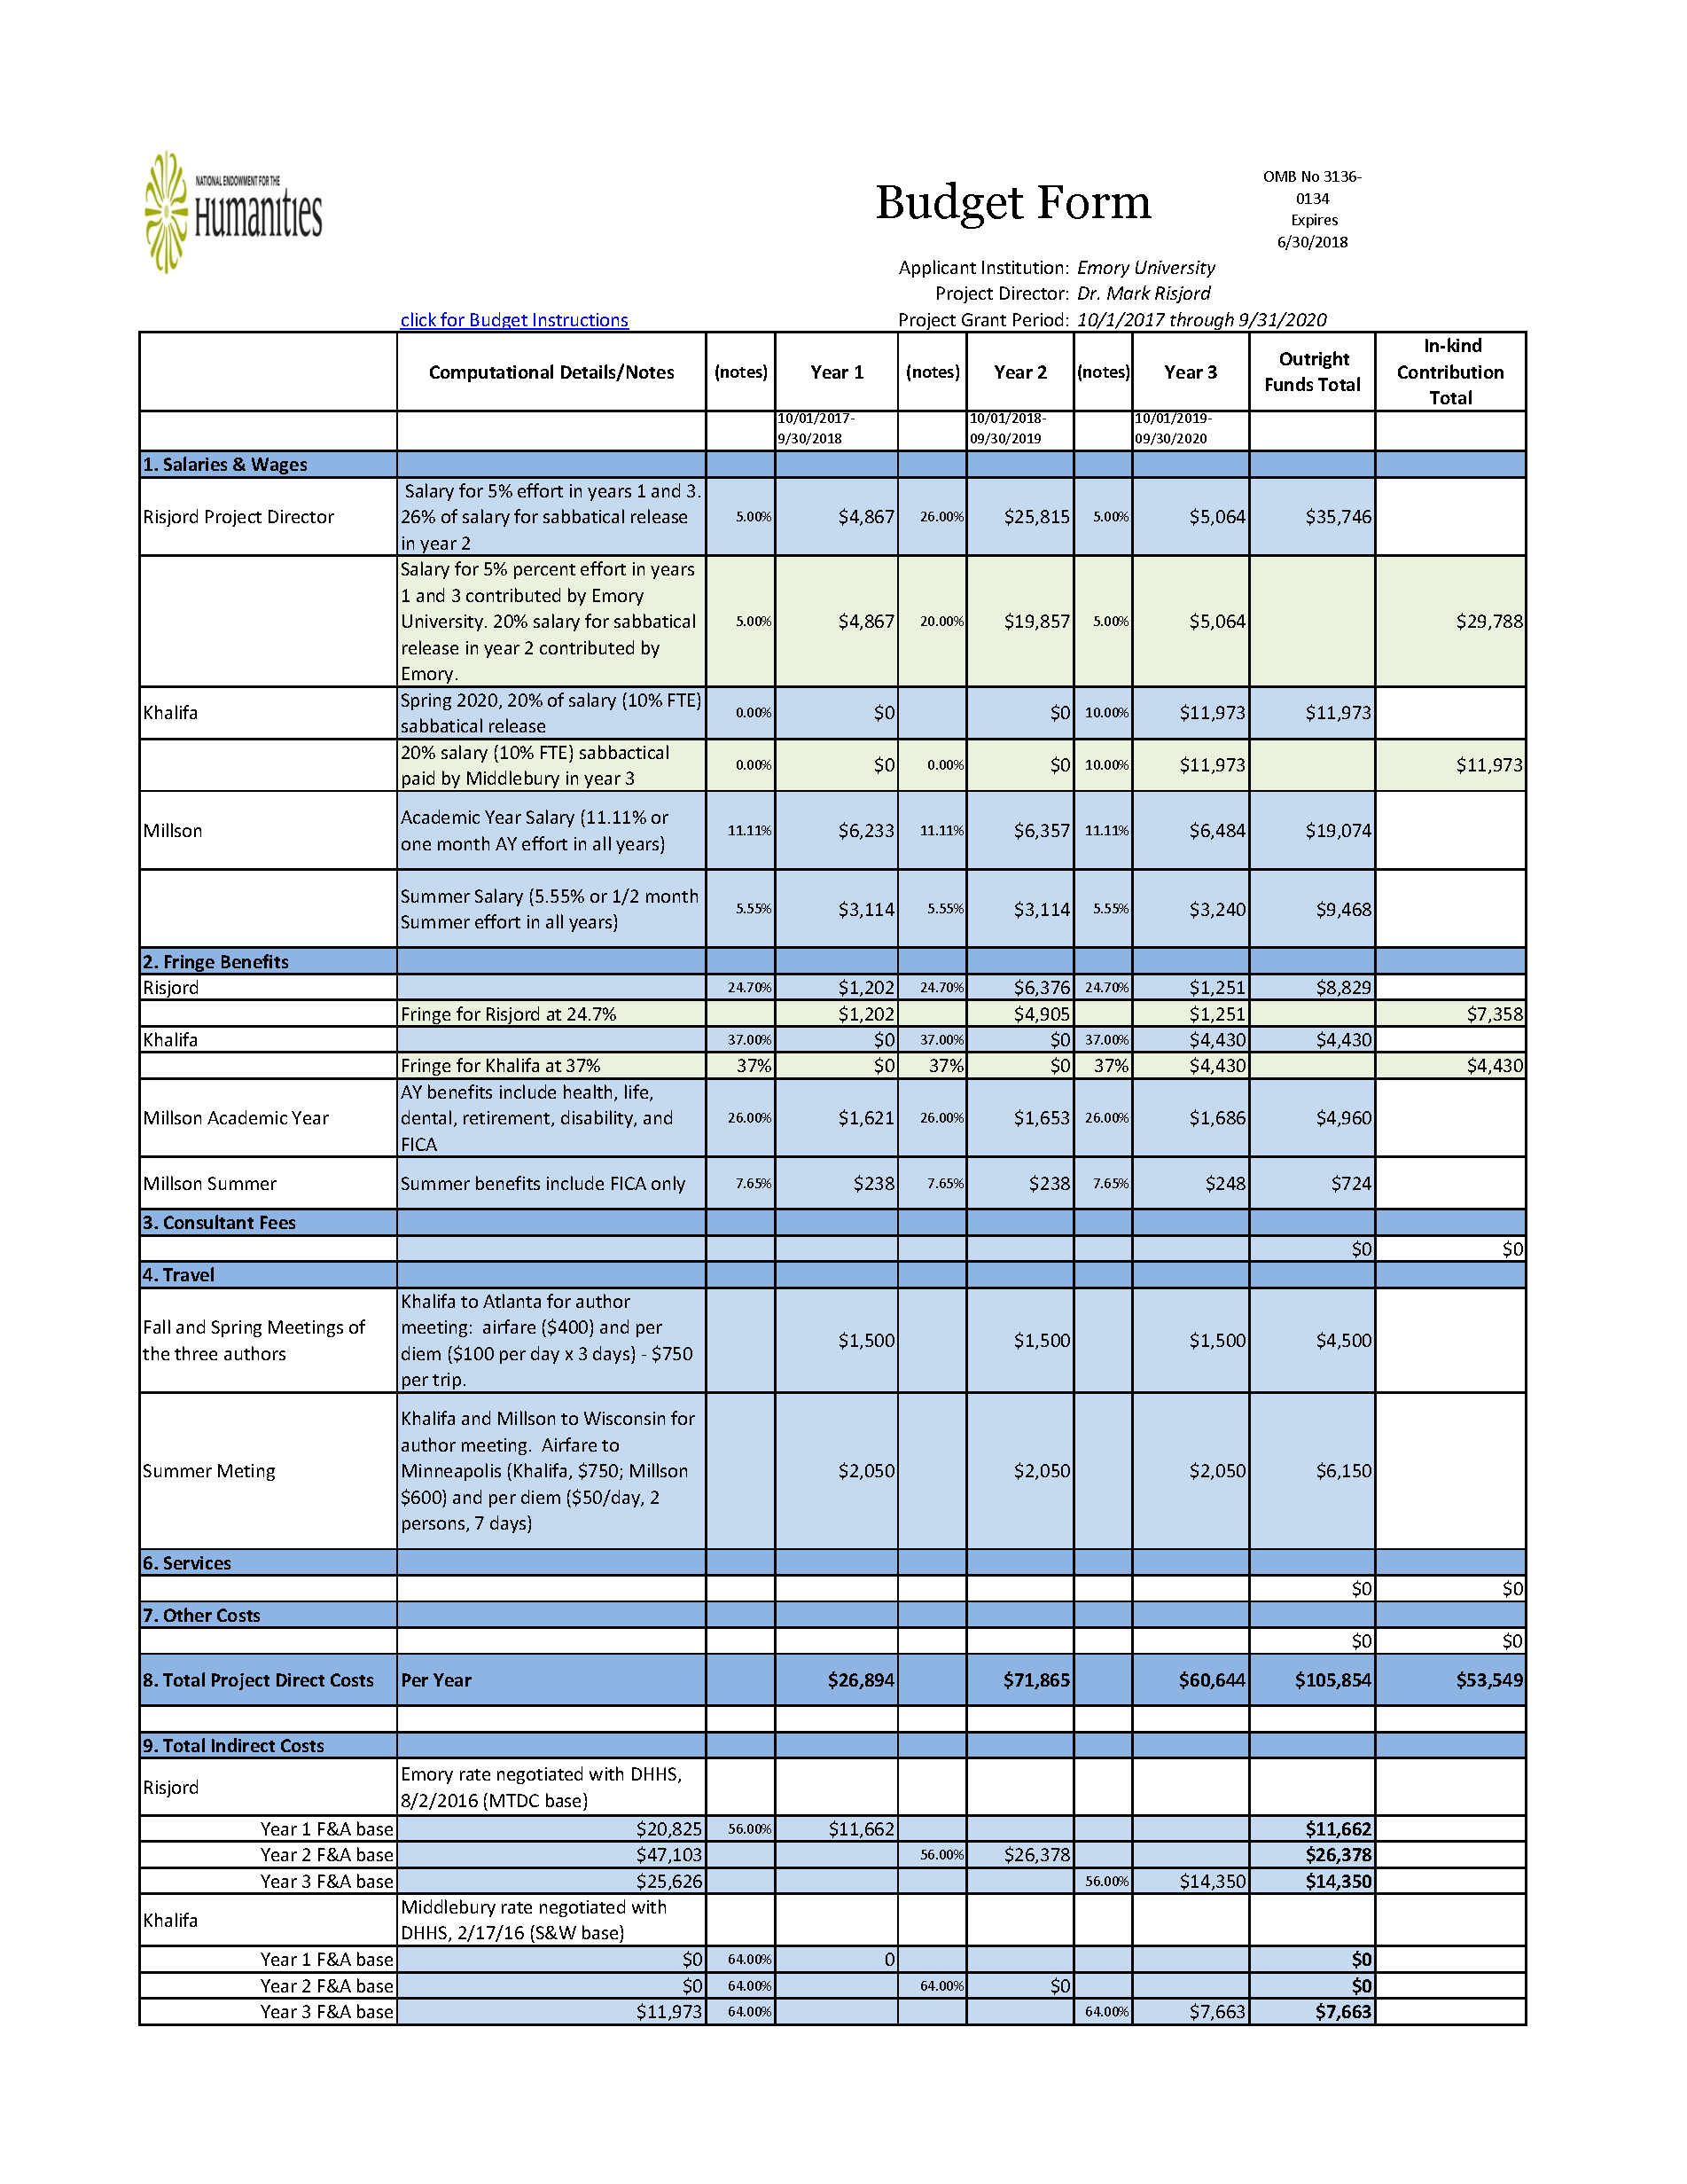
\includepdf[pages=1-2,pagecommand={\pagestyle{fancy}}]{NEH_Budget12012016}

%%%%%%%%%%%%%%%%%%%%%%%%%%%%%%%%%%%%%%%%%%%%%%%%%%%%%%%%%%%%%%%%%%%%%
%%%%%%%%%%%%%%%%%%%%%%%%%%%%%%%%%%%%%%%%%%%%%%%%%%%%%%%%%%%%%%%%%%%%%
\lhead{Bibliography}
\singlespacing

\section{Appendix 1: Bibliography}

\nocite{Douven1999,Harman1986a,Lipton2004,Lycan1988,Quine1970,Thagard1978,Thagard1992a,Thagard1999,Okasha2000,Poston2014,Psillos2009,Weisberg2009,Day1994,Fumerton1980,Salmon2001,Fraassen1989,Achinstein2001,Finetti1972,Earman1992a,Glymour1980,Howson1993,Kelly1996,Mayo1996,Norton2003,Norton2007,Ben-Menahem1990,Cartwright1983,Chakravartty2007,Hacking1983,Psillos1999,Stanford2006,Barnes1992,Bromberger1965,Gijsbers2007,Hempel1965,Friedman1974,Kitcher1989,Schurz1994,Morrison1999,Bechtel1993,Cartwright2007,Craver2007,Hall2004,Lewis1986,Reiss2015,Salmon1984,Strevens2008,Woodward2003,Baker2005,Batterman2002,Bokulich2011,Huneman2010,Lange2016,Risjord2005,Achinstein1983,Faye2007,Kitcher1987,Risjord2000,Fraassen1980,Sintonen1984,Boyd1983,Fine1986a,Kitcher2001,Ladyman2007,Laudan1981,Worrall1989,Chakravarttyforthcoming,Christensen2007,Elga2007,Kelly2005,Monton2007,Schoenfield2013,Fraassen1984,Fraassen2002,White2005a,Brandom1994,Brandom2008,Brandom2015,Peregrin2014,Hlobil2016,Kukla2009,Lange2000,Lange2009b,Millson2014,Millson2014a,Price2013,Rouse2002,Rouse2015,Sellars1963,Piazza2015,Piazza2016,DAgostino2015,Popper1963,Khalifa2006,Khalifa2010,Khalifaforthcomingb,Hintikka1995,Temple1988,Bromberger1966}

\vspace{3mm}
\textbf{{\large 1. Inference to the Best Explanation} (IBE)}\vspace{3mm}

\textbf{1.1. Positive Accounts and Defenses of IBE}

\printbibliography[keyword=IBE defense]

\textbf{1.2. Critiques of IBE}

\printbibliography[keyword=IBE_critique]

\textbf{1.3. IBE and Scientific Realism}

\printbibliography[keyword=IBE_Sci_Realism]

\textbf{1.4. Alternative Accounts of Induction}

\printbibliography[keyword=Induction]

\textbf{{\large 2. Explanation}}\vspace{3mm}

\textbf{2.1. Epistemic Accounts and their Critics}

\printbibliography[keyword=Epistem_Expl]

\textbf{2.2. Causal-Mechanical Accounts}

\printbibliography[keyword=Causal-Mechanical]

\textbf{2.3. Non-Causal Explanations}

\printbibliography[keyword=Non-Causal]

\textbf{2.4. Pragmatic Accounts and their Critics}

\printbibliography[keyword=Pragmatic]

\textbf{{\large 3. Scientific Progress, Realism, and Antirealism}}

\printbibliography[keyword=Realism]

\textbf{{\large 4. Permissive Conceptions of Rationality and their Critics}}

\printbibliography[keyword=permissivism]


\textbf{{\large 5. Philosophy of Language and Logic}}

\printbibliography[keyword=Language_and_Logic]


%%%%%%%%%%%%%%%%%%%%%%%%%%%%%%%%%%%%%%%%%%%%%%%%%%%%%%%%%%%%%%%%%%%%%
%%%%%%%%%%%%%%%%%%%%%%%%%%%%%%%%%%%%%%%%%%%%%%%%%%%%%%%%%%%%%%%%%%%%%
%change to single space with 12pt spacing between paragraphs
\lhead{Particpant CVs}
\clearpage

\section{Appendix 2: Participant CVs}

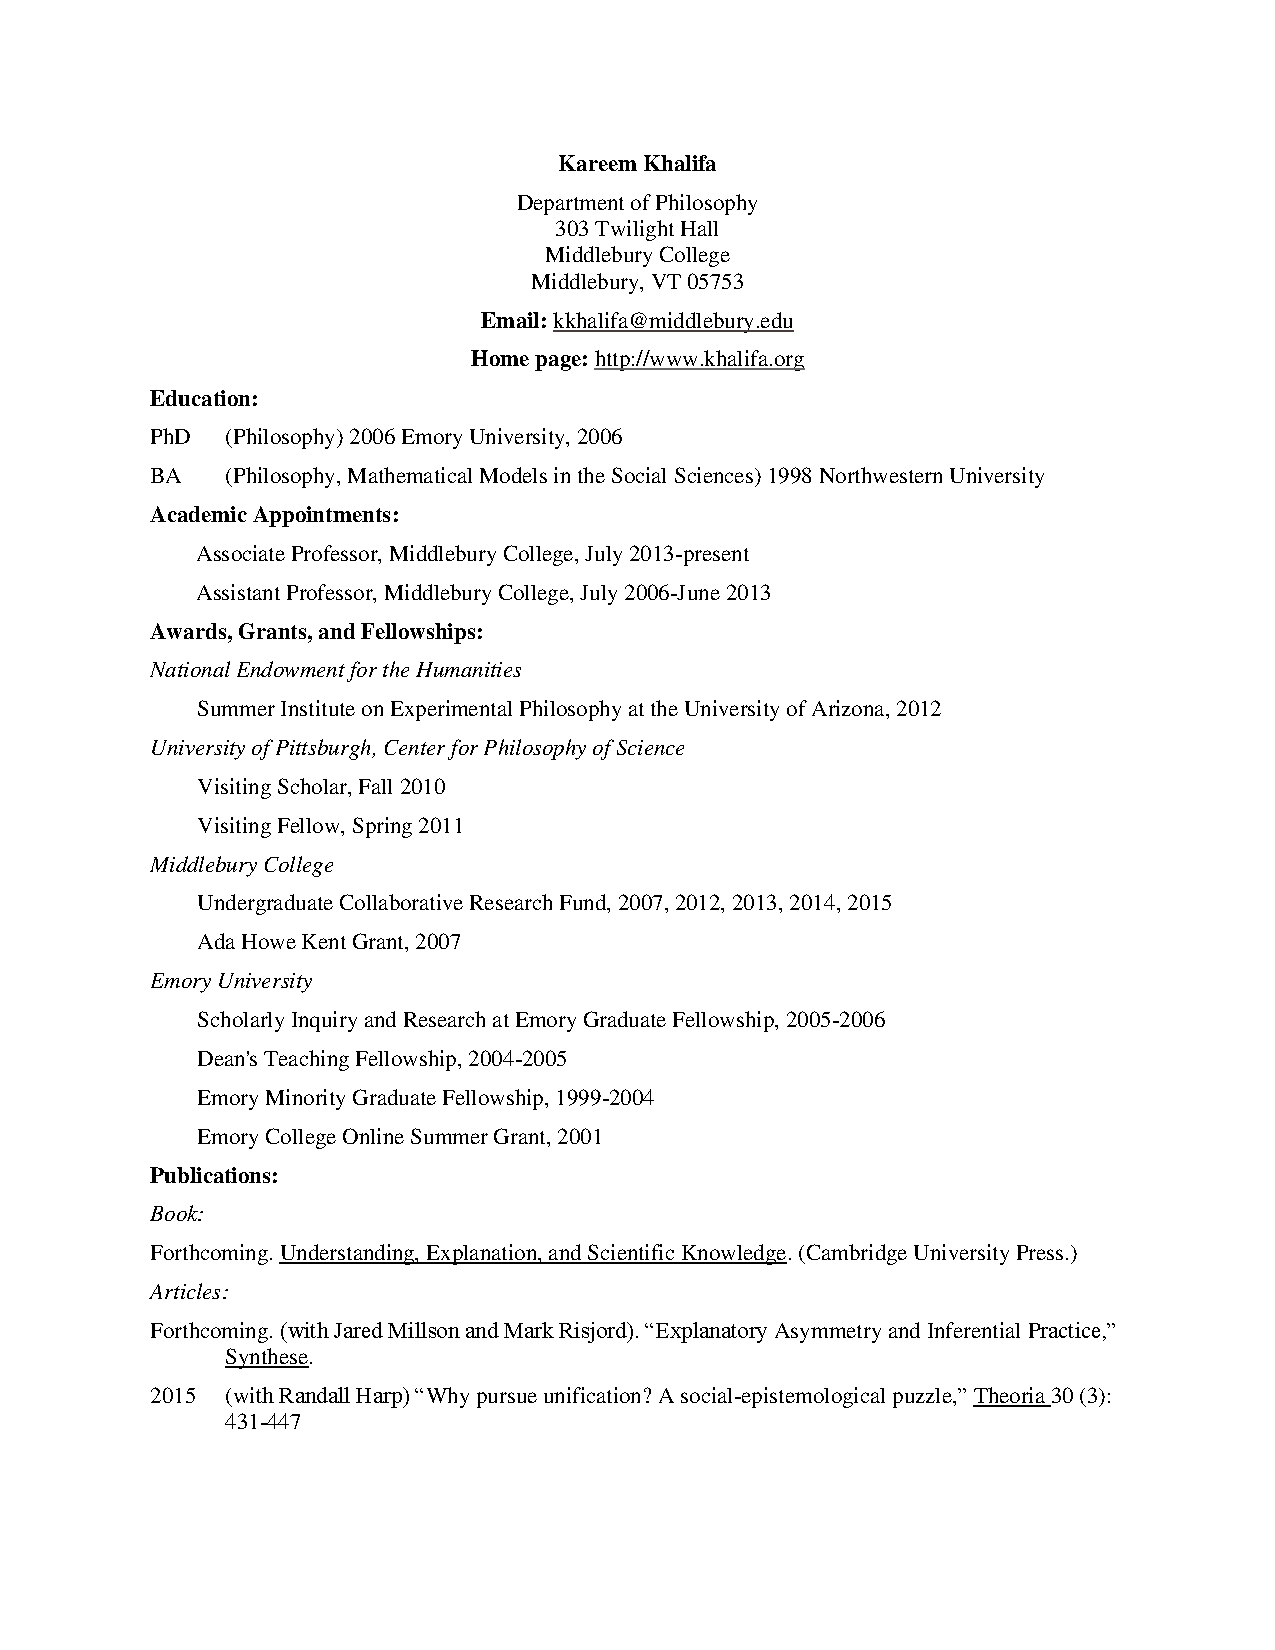
\includepdf[pages=1-5,pagecommand={\pagestyle{fancy}}]{All_CVs}


%%%%%%%%%%%%%%%%%%%%%%%%%%%%%%%%%%%%%%%%%%%%%%%%%%%%%%%%%%%%%%%%%%%%%
%%%%%%%%%%%%%%%%%%%%%%%%%%%%%%%%%%%%%%%%%%%%%%%%%%%%%%%%%%%%%%%%%%%%%

\lhead{Letters of Interest}
\section{Appendix 3: Letters of Interest}


\includepdf[pages=1]{Cambridge_Letter_of_Interest}


\includepdf[pages=1]{OUP_Letter_of_Interest}

%%%%%%%%%%%%%%%%%%%%%%%%%%%%%%%%%%%%%%%%%%%%%%%%%%%%%%%%%%%%%%%%%%%%%
%%%%%%%%%%%%%%%%%%%%%%%%%%%%%%%%%%%%%%%%%%%%%%%%%%%%%%%%%%%%%%%%%%%%%

\lhead{Grant History}
\section{Statement of History of Grants}




\clearpage
%%%%%%%%%%%%%%%%%%%%%%%%%%%%%%%%%%%%%%%%%%%%%%%%%%%%%%%%%%%%%%%%%%%%%
%%%%%%%%%%%%%%%%%%%%%%%%%%%%%%%%%%%%%%%%%%%%%%%%%%%%%%%%%%%%%%%%%%%%%

\end{document}
